% !TeX spellcheck = en_US

\documentclass[document.tex]{subfiles}

\begin{document}    
    \begin{frame}{Learning Outcomes}
        \textbf{After successfully completing the module, you will be able to:}
        \begin{itemize}
            \item help prepare and support management decisions through procurement, analysis and presentations of internal and external information by using different techniques and tools,
            \item determine the interactions between the different fields of a company/organisation when making management decisions and evaluate their effects, particularly concerning marketing, performance measurement or support of strategic decisions,
            \item explain "big data" and develop solution proposals for the processing of the data,
            \item determine which information might be relevant for which decision,
            \item examine as sources not only data and figures, but also unstructured texts,
            \item evaluate and apply fundamental methods from the field of "data science",
            \item substantiate findings determined by "data science" via statistical and mathematical bases.
        \end{itemize}
    \end{frame}

    \begin{frame}{Examination Modalities}
        \alert{\textbf{\textsc{Examinations}}}
        \vspace{-1mm}
        \begin{itemize}
            \item 60-minute \textbf{written examination} \textit{and}
            \item a \textbf{seminar paper} related to practical work in the field of data science.
        \end{itemize}

        \alert{\textbf{\textsc{Workload}}}
        \vspace{-1mm}
        \begin{itemize}
            \item Contact hours: 48 Teaching units
            \item Structured private studies: 109 hours
            \item Student Consulting/Practise Transfer: 55 hours
            \item \textbf{Overall workload: 200 hours}
        \end{itemize}
        	
        \textbf{Seminar paper and exam each count for 50\% of the module grade, both parts must receive an evaluation of at least 4.0. Remember to meet the deadlines! An extension will not be granted.}
    \end{frame}

    \begin{frame}{Written Examination}
        \begin{itemize}
            \item In the \textbf{60-minute written examination} you will be tested on the \textbf{fundamental theory and methodology that underpins data science} which means that you have to \textbf{learn this script and the things we will be actively discussing during the lectures by heart} - it will make fun and it is worth it.
            \item In most cases you will be asked either in \textbf{binary-choice} or in \textbf{free-text questions} what something is, what determines how it works, what the implications are when changing the determinants, what might cause problems and how can get those problems solved. For all the topics we will be discussing during the lectures \textbf{always ask} or answer those questions by yourself - this will be the best exam preparation at all.
            \item You will also have to work on a \textbf{case study exercise} in which you are requested to \textbf{evaluate a machine learning implementation} and give reasoned proposals in order to improve it. You will of course get a \textbf{mock exam} that will be discussed in the last lecture for better orientation and preparation.
            \item And even though we will be doing \textbf{math and programming} during the lectures, you are \textbf{neither required to do math nor programming in the written examination} - however, it is more than useful to know about it.
        \end{itemize}
    \end{frame}

    \begin{frame}{Seminar Paper: Prediction Competition I/II}
        \begin{itemize}
            \item Your job will be to act like a data scientist as you will be given a dataset in order to \textbf{develop a machine learning based model} that is capable of predicting in an accurate and robust manner whether or not a potential customer actually becomes a real customer.
            \item It will be up to you which method you want to choose for modeling: it could be either a simple \textbf{logistic regression model}, a \textbf{random forest} or even a more sophisticated \textbf{artificial neural network} - you will get to know the tools of the trade and how to use them appropriately.
            \item You will be also free to choose which features of the dataset you want to use in your model and which not and whether and in what manner you want to \textbf{preprocess} those features in terms of cleaning, aggregating, transforming, engineering or whatever else comes to your mind.
            \item The seminar paper which achieves the \textbf{lowest prediction error} on the features of a dataset whose actual outcome will be unknown to you will be receiving the \textbf{best grade in this partial aspect}.
        \end{itemize}
    \end{frame}

    \begin{frame}{Seminar Paper: Prediction Competition II/II}
        \alert{\textbf{\textsc{General conditions}}}
        \vspace{-1mm}
        \begin{itemize}
            \item What you will be \textbf{uploading to the online campus} at the end of the semester is your \textbf{code}, a file with your \textbf{prediction results} and a \textbf{written seminar paper}.
            \item As the major focus is put on the \textbf{practical work}, the seminar paper must have \textbf{not less than four and not more than five text pages} and must contain \textbf{only those four bullet points}: an introduction (with problem definition and practical relevance), a theoretical elaboration on the chosen model, a report on how the data has been preprocessed and modeled plus an evaluation of the validation results.
            \item You may of course \textbf{form teams with up to four people} to work out a solution. However, the \textbf{seminar paper must be written independently} and its \textbf{title page must list all team members}.
        \end{itemize}
        \alert{\textbf{\textsc{Evaluation}}}
        \vspace{-1mm}
        \begin{itemize}
            \item Part of the evaluation is the \textbf{appropriateness in data preprocessing, modeling and model selection} as well as detailedness, reasoned explanations and interpretations.
            \item If all those \textbf{items are graded at least 4.0} then \textbf{one third of the grade} is determined by the \textbf{goodness of the predictions}. This means that the seminar paper with the worst predictions gets a 4.0 in this particular aspect whereas the best seminar paper gets a 1.0. All other grades are interpolated between those.
        \end{itemize}
    \end{frame}

    \begin{frame}{20th Annual KDnuggets Software Poll}
        \begin{figure}
            \label{fig:kdnuggets-poll-2019}
            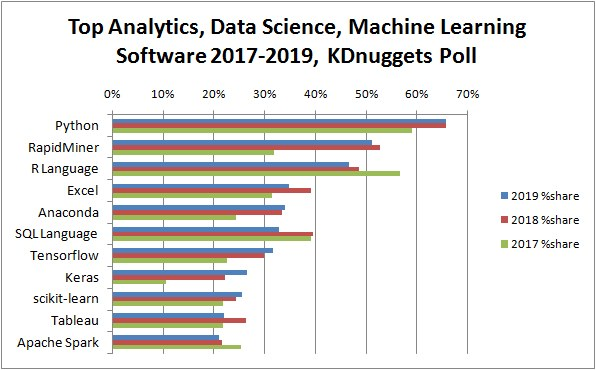
\includegraphics[width=0.7\textwidth]{figures/external/kdnuggets-poll-2019.jpg}
        \end{figure}
    \end{frame}
    
    \begin{frame}{Jupyter Programming Environment}
        \begin{alertblock}{\textsc{Google Colaboratory}}
            Google Colaboratory is a Jupyter notebook environment bases on Python 3.6. used for machine learning education and research with Python. It is free to use and requires no setup. 
            \vspace{-1mm}
            
            \textsc{\textbf{Link:}} \href{https://colab.research.google.com/}{https://colab.research.google.com/}
        \end{alertblock}
        \begin{alertblock}{\textsc{Kaggle}}  
            Kaggle offers a no-setup, customizable, Jupyter Notebooks environment. Access free GPUs and a huge repository of community published data \& code.
            \vspace{-1mm}

            \textsc{\textbf{Link:}} \href{https://www.kaggle.com/}{https://www.kaggle.com/}
        \end{alertblock}
        \begin{alertblock}{\textsc{Anaconda}}
            If you want to setup a local Python programming environment, you should use the Anaconda distribution as it is one of the most popular Python data science distributions and is therefore properly documented.
            \vspace{-1mm}
            
            \textsc{\textbf{Link:}} \href{https://www.anaconda.com/}{https://www.anaconda.com/}
        \end{alertblock}
    \end{frame}

    \begin{frame}{Auxiliary Materials}
        You will find all \textbf{datasets} we will be using during the lectures in the accompanying \textbf{GitHub repository} available at \href{https://github.com/saschaschworm/big-data-and-data-science}{https://github.com/saschaschworm/big-data-and-data-science}. There you will also find all \textbf{solutions to the development exercises} you will be conducting in class as \textbf{Jupyter notebook} as well as a \textbf{minimum working example} for the seminar paper.
    \end{frame}

    \begin{frame}{Literature Recommendations}
        \begin{minipage}{0.1\textwidth}
            \begin{figure}[H]
                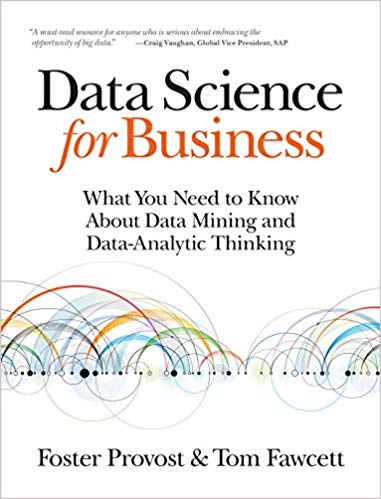
\includegraphics[height=0.2\textheight, width=0.9\textwidth, left]{assets/book-covers/provost2013.jpg}
            \end{figure}
        \end{minipage}
        \begin{minipage}{0.32\textwidth}
            \footnotesize Foster Provost, Tom Fawcett \normalsize \\[-0.5mm]
            \small \textbf{Data Science for Business} \normalsize \\
            \tiny First Edition, 2013, Sebastopol: O'Reilly \normalsize
        \end{minipage}
        \begin{minipage}{0.1\textwidth}
            \begin{figure}[H]
                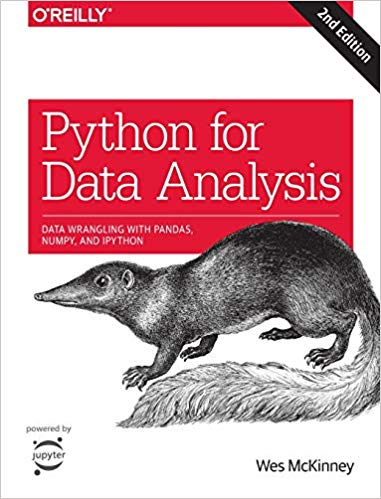
\includegraphics[height=0.2\textheight, width=0.9\textwidth, left]{assets/book-covers/mckinney2017.jpg}
            \end{figure}
        \end{minipage}
        \begin{minipage}{0.39\textwidth}
            \footnotesize Wes McKinney \normalsize \\[-0.5mm]
            \small \textbf{Python for Data Analysis} \\[-0.8mm]
            Data Wrangling with Pandas, NumPy, and IPython \normalsize \\
            \tiny Second Edition, 2017, Sebastopol: O'Reilly \normalsize
        \end{minipage}
        
        \begin{minipage}{0.1\textwidth}
            \begin{figure}[H]
                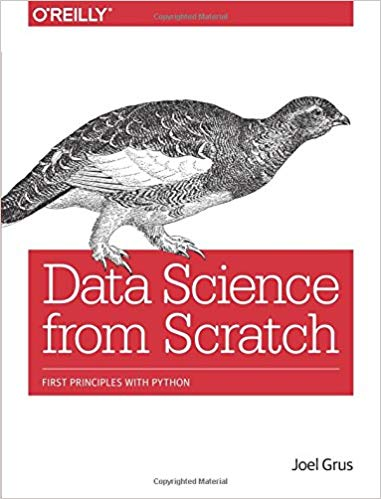
\includegraphics[height=0.2\textheight, width=0.9\textwidth, left]{assets/book-covers/grus2015.jpg}
            \end{figure}
        \end{minipage}
        \begin{minipage}{0.32\textwidth}
            \footnotesize Joel Grus \normalsize \\[-0.5mm]
            \small \textbf{Data Science from Scratch} \\[-0.8mm]
            First Principles with Python \normalsize \\
            \tiny First Edition, 2015, Sebastopol: O'Reilly \normalsize
        \end{minipage}
        \begin{minipage}{0.1\textwidth}
            \begin{figure}[H]
                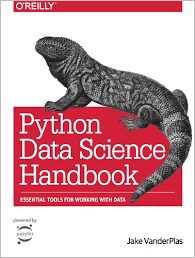
\includegraphics[height=0.2\textheight, width=0.9\textwidth, left]{assets/book-covers/vanderplas2016.png}
            \end{figure}
        \end{minipage}
        \begin{minipage}{0.39\textwidth}
            \footnotesize Jake VanderPlas \normalsize \\[-0.5mm]
            \small \textbf{Python Data Science Handbook} \\[-0.8mm]
            Essential Tools for Working with Data \normalsize \\
            \tiny First Edition, 2016, Sebastopol: O'Reilly \normalsize
        \end{minipage}
        
        \begin{minipage}{0.1\textwidth}
            \begin{figure}[H]
                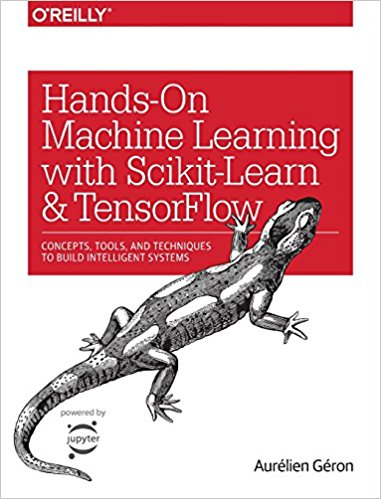
\includegraphics[height=0.2\textheight, width=0.9\textwidth, left]{assets/book-covers/geron2017.jpg}
            \end{figure}
        \end{minipage}
        \begin{minipage}{0.32\textwidth}
            \footnotesize Aurélien Géron \normalsize \\[-0.5mm]
            \small \textbf{Hands-On Machine Learning} \\[-0.8mm]
            \textbf{with Scikit-Learn and TensorFlown} \normalsize \\
            \tiny First Edition, 2017, Sebastopol: O'Reilly \normalsize
        \end{minipage}
        \begin{minipage}{0.1\textwidth}
            \begin{figure}[H]
                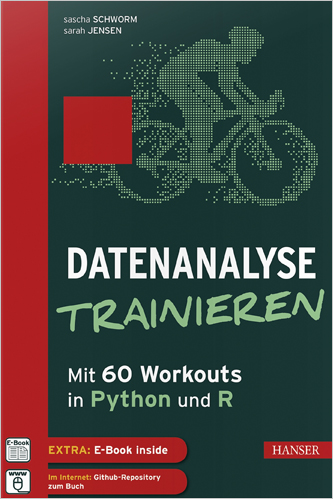
\includegraphics[height=0.2\textheight, width=0.9\textwidth, left]{assets/book-covers/schworm2019.jpg}
            \end{figure}
        \end{minipage}
        \begin{minipage}{0.39\textwidth}
            \footnotesize Sascha Schworm, Sarah Jensen \normalsize \\[-0.5mm]
            \small \textbf{Datenanalyse trainieren} \\[-0.8mm]
            60 Workouts in Python und R \normalsize \\
            \tiny First Edition, München: Hanser, Available: Nov 2019 \normalsize
        \end{minipage}
    \end{frame}

    \begin{frame}{Course Outline}
        \begin{minipage}[t]{.5\textwidth}
            \textbf{Lecture: Big Data \& Data Science}
            \tableofcontents[hideallsubsections]       
            \vspace{4.22mm}
            \textbf{Introduction to Data Science and Machine Learning}
            \vspace{1.22mm}
            \tableofcontents[hideallsubsections, sections={1-7}, part=1]  
        \end{minipage}%
        \begin{minipage}[t]{.5\textwidth}
            \textbf{Methods and Models in Machine Learning}
            \tableofcontents[hideallsubsections, sections={5-9}, part=2]
        \end{minipage}
    \end{frame}
\end{document}